\documentclass{article}
\usepackage[UTF8, heading = false, scheme = plain]{ctex}

\usepackage{geometry}
\geometry{b5paper,left=2cm,right=2cm,top=2cm,bottom=2cm}

\usepackage{color}
\usepackage{amsfonts}
\usepackage{amsmath}

\linespread{1.5}

\usepackage[colorlinks,
            linkcolor=red,
            anchorcolor=blue,
            citecolor=green
            ]{hyperref}

\usepackage{listings}
\usepackage{fontspec}
\usepackage{graphicx}
\usepackage{algorithmic}
\newfontfamily\monaco{Monaco}
\definecolor{dkgreen}{rgb}{0,0.6,0}
\definecolor{gray}{rgb}{0.5,0.5,0.5}
\definecolor{mauve}{rgb}{0.58,0,0.82}
\lstset{ %
  basicstyle=\footnotesize\monaco,       % the size of the fonts that are used for the code
  numbers=left,                   % where to put the line-numbers
  numberstyle=\footnotesize\monaco\color{gray},  % the style that is used for the line-numbers
  numbersep=5pt
  stepnumber=1,                   % the step between two line-numbers. If it's 1, each line
                                  % will be numbered
  numbersep=5pt,                  % how far the line-numbers are from the code
  backgroundcolor=\color{white},      % choose the background color. You must add \usepackage{color}
  showspaces=false,               % show spaces adding particular underscores
  showstringspaces=false,         % underline spaces within strings
  showtabs=false,                 % show tabs within strings adding particular underscores
  frame=lines,                   % adds a frame around the code
  rulecolor=\color{black},        % if not set, the frame-color may be changed on line-breaks within not-black text (e.g. commens (green here))
  tabsize=4,                      % sets default tabsize to 2 spaces
  captionpos=t,                   % sets the caption-position to bottom
  breaklines=true,                % sets automatic line breaking
  breakatwhitespace=false,        % sets if automatic breaks should only happen at whitespace
  title=\lstname,                   % show the filename of files included with \lstinputlisting;
                                  % also try caption instead of title
  keywordstyle=\color{blue},          % keyword style
  commentstyle=\color{dkgreen},       % comment style
  stringstyle=\color{mauve},         % string literal style
  escapeinside={\%*}{*)},            % if you want to add LaTeX within your code
  morekeywords={*,...}               % if you want to add more keywords to the set
}

\usepackage{amssymb} 
\usepackage{amsmath}
\usepackage[ruled,vlined]{algorithm2e}

\setlength{\parindent}{2em}

\renewcommand{\G}{\mathbb{G}}
\newcommand{\Z}{\mathbb{Z}}
\newcommand{\Q}{\mathbb{Q}}
\newcommand{\F}{\mathbb{F}}

\newcommand{\Sbox}{\textsf{Sbox}}
\newcommand{\code}[1]{\lstinline!#1!}

\newcommand{\CKDpriv}{\textsf{CKDpriv}}
\newcommand{\CKDpub}{\textsf{CKDpub}}

%%%%%%%处理下划线:_%%%%%%%%%
\usepackage{underscore}
%%%%%%%处理下划线:_%%%%%%%%%

\setlength{\parindent}{2.1em}

%%%设置页眉和页码格式
\usepackage{fancyhdr}
\newcommand{\makeheadrule}{%
\rule[0.85\baselineskip]{\headwidth}{0.5pt}\vskip-.8\baselineskip}%1.5 0.4->0.5
\makeatletter
\renewcommand{\headrule}{%
{\if@fancyplain\let\headrulewidth\plainheadrulewidth\fi
\makeheadrule}}
\makeatother
\pagestyle{fancy}
\fancyhf{}
\fancyhead[r]{\textit{Crypto In Action}}
\fancyfoot[C]{--{~\thepage~}--}
%%%设置页眉和页码格式结束

\usepackage{color}
\newcommand{\red}{\textcolor{red}}
\newcommand{\blue}{\textcolor{blue}}

\begin{document}

\title{Paillier: Theory and Implementation}
\author{longcpp \\ \small{longcpp9@gmail.com}}

\maketitle

Pascal Paillier在其1999年的论文
``Public-Key Cryptosystems Based on Composite Degree Residuosity Classes''
中引入了Paillier公钥加密机制, 其安全性由合成剩余类(Composite Residuosity Classes)
相关的困难问题保证. Paillier的特殊之处是在概率加密的基础之上保留了加法同态的特性.
这一特性被广泛应用于构造各类密码协议, 例如近年来提出应用于数字货币领域的
的两方ECDSA签名协议和多方阈值ECDSA签名协议.

与其他公钥加密机制一样, Paillier公钥加密机制也由密钥生成(Key Generation)
加密(Encryption)和解密(Decryption)三个算法组成.
三个算法的详细计算过程在图~\ref{fig-paillier}~中展示, 
图~\ref{fig-paillier}~截取自Sigrun Goluch的毕业论文
``The development of homomorphic cryptography''. 
为了理解图~\ref{fig-paillier}~中展示的过程,需要先介绍\textbf{Carmichael函数}的概念.
对于正整数$n$, \textbf{Carmichael函数$\lambda(n)$}表示满足下面要求的最小的正整数$t$:
$$x^t \equiv 1 ~\textsf{mod}~ n, ~\text{其中}~ x \in \Z ~\text{并且}~ \textsf{gcd}(x, n) = 1.$$
对于素数$p$, 根据费马小定理可知$\lambda(p) = \varphi(p) = p-1$, 其中$\varphi$表示欧拉函数.
根据代数基本定理可以对任意整数$n$做唯一分解,记为$n = p_1^{a_1}p_2^{a_2}\cdots p_k^{a_k}$,
其中$p_1, p_2, \cdots, p_k$为互不相同的素数. 
R. D. Carmichael在1912年给出了求解$\lambda(n)$的计算公式($\textsf{lcm}$表示最小公倍数): 
\begin{equation*}
\lambda(n) = \textsf{lcm}\left(\lambda\left(p_1^{a_1}\right), \lambda\left(p_2^{a_2}\right), \cdots, \lambda\left(p_k^{a_k}\right)\right),
\lambda(p_i^{a_i}) = 
\left\{
\begin{array}{l}
2^{a_i - 2}, ~\text{for}~ p_i = 2, a_i > 2\\
(p_i - 1)p_i^{a_i - 1}, ~\text{otherwise}~\\
\end{array}
\right.
\end{equation*}
Paillier公钥加密机制中仅关心$n = pq$且$p, q$为大素数的情形, 
根据上式有$\lambda(n)=\textsf{lcm}(p-1, q-1)$, 并且
$\lambda(n^2) = \textsf{lcm}(p(p-1), q(q-1)) = n\cdot\textsf{lcm}(p-1, q-1) = n\lambda(n)$.

密钥生成算法$\textsf{KeyGen}$的输入为两个大素数$p$, $q$,
而$g$则是从$\Z_{n^2}^*$中选取的满足
$\textsf{gcd}\left(L\left(g^\lambda \mod n^2\right), n\right) = 1$
的元素, 其中的映射$L: \Z_{n^2}^* \rightarrow \Z_n$定义为$L(u) = \blue{\frac{u-1}{n}}$.
值得注意的是,与通常的密码学构造书写规范不同的是,
映射$L$的定义中$\blue{\frac{u-1}{n}}$的含义是,计算$u-1$除以$n$的商,
而非在$\Z_{n^2}^*$中计算$u-1$乘以$n$的逆.

\begin{figure}[h]
\centering
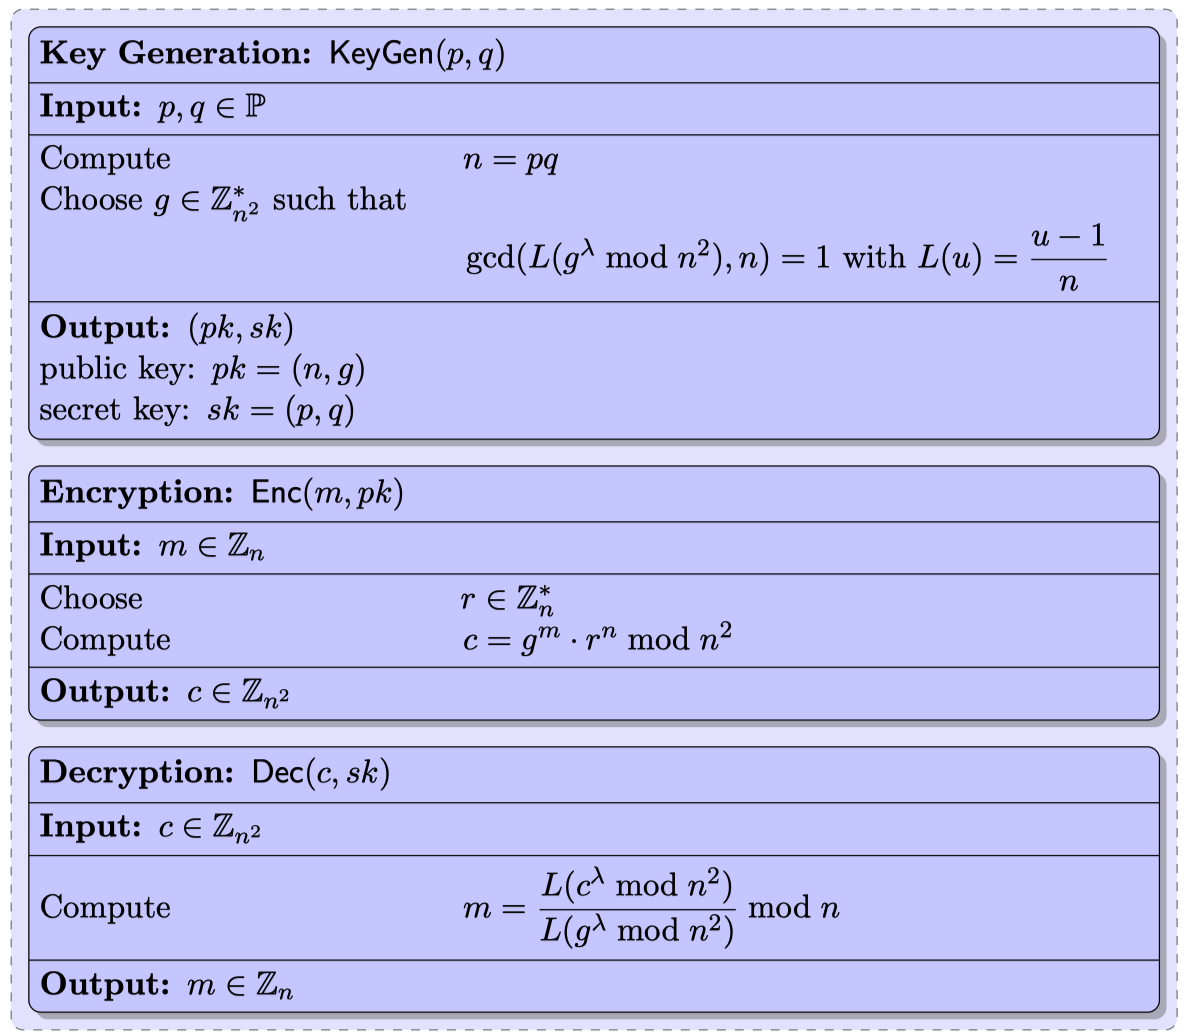
\includegraphics[width=\textwidth]{paillier.png}
\caption{Paillier公钥加密机制}\label{fig-paillier}
\end{figure}


\end{document}

